
Learning from interactions with users is ubiquitous in modern customer-facing platforms, from product recommendations to web search to content selection to fine-tuning user interfaces. Many platforms purposefully implement \emph{exploration}: making potentially suboptimal choices for the sake of acquiring new information.
Online platforms routinely deploy A/B tests, and are increasingly adopting  more sophisticated exploration methodologies based on \emph{multi-armed bandits}, a well-known framework for exploration and making decisions under uncertainty.


%~\cite{KohaviAB-2015,KohaviLSH09}

In this paper, we initiate a study of the interplay between \exploration and \competition. Platforms that engage in exploration typically need to compete against one another; most importantly, they compete for users. This creates a tension:
%between \exploration and \competition.
while exploration may be essential for improving the service tomorrow, it may degrade quality and make users leave \emph{today}, in which case there will be less users to learn from. This may further degrade the platform's performance relative to competitors who keep learning and improving from \emph{their} users, and so forth. Taken to the extreme, such dynamics may create a ``death spiral" effect when the vast majority of customers eventually switch to competitors. Users therefore serve three distinct roles: they are customers that generate revenue, they are sources of data for learning, and they are self-interested agents who choose among the competing systems.

The main high-level question that we focus on in this paper is:
\begin{align}\label{eq:main-Q}
\textbf{How does competition incentivize the adoption of better exploration algorithms?}
\end{align}

\noindent This translates into a number of more concrete questions. While it is commonly assumed that better technology always helps, is this so under competition? Does increased competition lead to higher consumer welfare? How significant are ``data feedback loops" --- when more data leads to more users, which leads to even more data, etc. --- and how they relate to the anti-trust considerations? Finding formalizations that admit meaningful answers is a major part of the overall challenge.




To answer these questions, we study complex interactions between platforms' learning dynamics and users' self-interested behavior. The choice of a particular technology (exploration algorithm) is no longer an abstract, static choice with a predetermined outcome for the platform. Instead, we model the algorithms explicitly, and investigate how they play out in competition over an extended period of time.


%\footnote{This is a fundamental question which is part of a larger policy discussion around whether data can serve as an indirect network effect and lead to similar ``market tipping" results as is standard in the literature on competition in markets with network effects (see \cite{jullien2019economics} for a policy oriented discussion of this).}

% the extent to which the game between the two principals is competitive
% degree of innovation that these models incentivize.
% the extent to which agents make rational decisions


%\subsection{Our model}
%\label{sec:intro-model}

\subsection{Our model: competing bandits}
\label{sec:intro-model}

%We investigate these questions with
\xhdr{Competition game.} We consider a stylized duopoly model where two firms commit to exploration strategies and compete for a stream of consumers. We define a game in which two firms (\emph{principals}) simultaneously engage in exploration and compete for users (\emph{agents}). These two processes are interlinked, as exploration decisions are experienced by users and informed by their feedback. We need to specify several conceptual pieces: how the principals and agents interact, what is the machine learning problem faced by each principal, and what is the information structure. Each piece can get rather complicated in isolation, let alone jointly, so we strive for simplicity. Thus, the key features of our model are as follows:

\begin{itemize}

\item A new agent arrives in each round $t=1,2, \ldots$, and chooses among the two principals. The principal chooses an action (\eg a list of web search results to show to the agent), the user experiences this action, and reports a reward. All agents have the same ``decision rule" for choosing among the principals given the available information.

\item Each principal faces a basic and well-studied version of the multi-armed bandit problem: for each arriving agent, it chooses from a fixed set of actions  (a.k.a. \emph{arms}) and receives a reward drawn independently from a fixed distribution specific to this action. The reward distributions are initially unknown (but can be estimated over time from the data).

\item Principals simultaneously announce their bandit algorithms before round $1$, and cannot change them afterwards.  Each principal's objective is to maximize its market share (the fraction of users choosing this principal). Each principal only observes agents that chose this principal.
%, but may have access to each platforms' reputation score (more on this in    Section~\ref{sec:intro-discussion}).
\end{itemize}

\noindent We investigate several model variants within this framework, where we vary agents' decision rule and/or give a first-mover advantage to one of the principals. In all variants, agents have little or no information about other agents' choices and rewards.

%We consider two model variants, which determine agents' decision rule and their information sets. In \emTheoryModel, there is a common Bayesian prior on the reward distributions. Agents do not receive any other information and choose between the principals using their knowledge of $t$ and the principals' algorithms. In \emExptsModel, agents have access to a reputation score for each principal, which is a sliding window average of the rewards experienced by previous agents that have visited this principal. The former variant used for the theoretical results, the latter for simulations.

\xhdr{Technology: multi-armed bandit algorithms.}
To flesh out \eqref{eq:main-Q}, let us elaborate what we mean by `better' bandit algorithms. In general, comparisons between bandit algorithms are rather subtle, as some algorithms may be better for some problem instances and/or time intervals, and worse for some others.

We distinguish three classes of bandit algorithms, based on
the prevalent intuition in the area. The distinction concerns the way in which they resolve the fundamental tradeoff between  exploration and \emph{exploitation} (making optimal myopic decisions using the available data). Going from more primitive to more sophisticated, these three classes are as follows:

\begin{itemize}
\item \emph{Greedy algorithms} that strive to maximize the reward for the next round given the available information. Thus, they always ``exploit" and never explicitly ``explore".


\item \emph{Exploration-separating algorithms}
 that separate exploration and exploitation: essentially, each round is dedicated to one and completely ignores the other.

\item \emph{Adaptive-exploration} algorithms that combine exploration and exploitation, and gradually sway the exploration choices towards more promising alternatives.
\end{itemize}

In isolation, \ie in the absence of competition, these classes are fairly well-understood. Greedy algorithms are terrible for a wide variety of problem instances, precisely because they never explore. Exploration-separated algorithms learn at a reasonable but mediocre rate across all problem instances. Adaptive-exploration algorithms are optimal in the worst case, and exponentially improve for ``easy" problem instances. Generally,  ``better" algorithms are better in the long run, but could be worse initially.



\subsection{Our Results}
\label{sec:intro-results}

We offer a mix of theoretical results and numerical simulations. We are mainly interested in qualitative differences between the three classes of algorithms in Section~\ref{sec:intro-model}. For numerical simulations, we pick one representative algorithm from each class. For theoretical results, we allow arbitrary algorithms and focus on asymptotic differences in the algorithms' performance.

\xhdr{Theoretical results.}
%We endow agents with Bayesian rationality, a common modeling approach for a theoretical investigation.
We consider a basic Bayesian model. We posit that agents have a common Bayesian prior on reward distributions, and know the principals' algorithms. For simplicity, agents do not receive any information about the previous agents' choices and rewards. Each agent knows the round (s)he arrives in, computes the Bayesian-expected reward for each principal, and use these two numbers to decide which principal to choose. We refer to this variant as the \emph{\TheoryModel}.

Our results depend crucially on the agents' decision rule.
\begin{itemize}

\item The most obvious decision rule maximizes the Bayesian-expected reward; we refer to it as \HardMax. We find that \HardMax is not conducive to adopting better algorithms: each principal's dominant strategy is to choose the greedy algorithm. Further, we show that \HardMax is very sensitive to tie-breaking: if the tie-breaking is probabilistically biased in favor of one principal, then this principal has a simple ``winning strategy" no matter what the other principal does.

\item We dilute the \HardMax agents with a small fraction of ``random agents" who choose a principal uniformly at random. We call this model \HardMaxRandom. We find that better algorithms help in a big way: a sufficiently better algorithm is guaranteed to win all non-random agents after an initial learning phase. However, there is a substantial caveat: one can defeat any algorithm by interleaving it with the greedy algorithm. This has two undesirable corollaries: a better algorithm may sometimes lose in competition, and a pure Nash equilibrium typically does not exist.

\item We further relax the decision rule so that the probability of choosing a given principal varies smoothly as a function of the difference between  principals' Bayesian-expected rewards; we call it \SoftMaxRandom. For this model, the ``better algorithm wins" result holds under much weaker assumptions on what constitutes a better algorithm. This is the most technical result of the paper. The competition in this setting is necessarily much more relaxed: typically, both principals attract approximately half of the agents as time goes by (but a better algorithm would attract slightly more).
\end{itemize}

All results extend to a much more general version of the multi-armed bandit problem in which the principal may observe additional feedback before and/or after each decision, as long as the feedback distribution does not change over time. In most results, principal's utility may depend on both the market share and agents' rewards.

\begin{figure}
\begin{center}
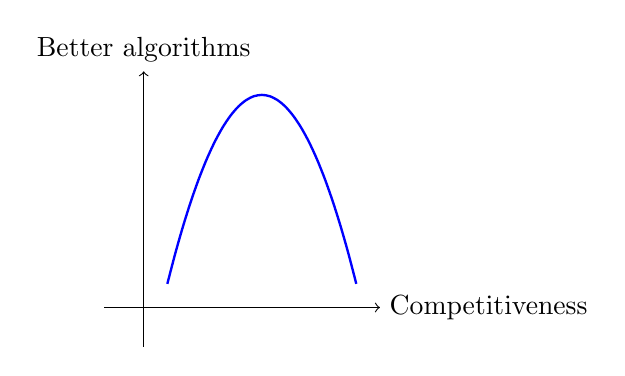
\begin{tikzpicture}
      \draw[->] (-.5,0) -- (3,0) node[right] {Competitiveness};
      \draw[->] (0,-.5) -- (0,3) node[above] {Better algorithms};
      \draw[scale=0.6,domain=0.5:4.5,smooth,variable=\x,blue, line width=0.3mm] plot ({\x},{4.5 - (\x - 2.5)^2});
      % \draw[scale=0.5,domain=-3:3,smooth,variable=\y,red]  plot ({\y*\y},{\y});
 \end{tikzpicture}

\caption{Inverted-U relationship between competitiveness and algorithms.}
\label{fig:inverted-U}
\end{center}
\end{figure}


\xhdr{Economic interpretation: the inverted-U relationship.}
Interpreting the adoption of better algorithms as ``innovation", our findings can be framed in terms of the inverted-U relationship between competition and innovation, as in Figure~\ref{fig:inverted-U}.%
\footnote{Here, ``innovation" refers to adoption of a better technology at a substantial R\&D expense to a given firm. It is not salient whether similar ideas and/or technologies already exist elsewhere. Adoption of exploration algorithms tends to require substantial R\&D effort in practice, even if the algorithms themselves are well-known in the research literature \citep[\eg see][]{DS-arxiv}.}
This is a well-established concept in the economics literature, dating back to \cite{Schumpeter-42}, whereby too little or too much competition is bad for innovation, but intermediate levels of competition tend to be better \citep[\eg][]{Aghion-QJE05,Vives-08}.

Our decision rules differ in terms of rationality: from fully rational decisions with \HardMax to relaxed rationality with \HardMaxRandom to an even more relaxed rationality with \SoftMaxRandom. The same distinctions also control the severity of competition between the principals: from cut-throat competition with \HardMax to a more relaxed competition with \HardMaxRandom, to an even more relaxed competition with \SoftMaxRandom. Indeed, with \HardMax you lose all customers as soon as you fall behind in performance, with \HardMaxRandom you get some small market share no matter what, and with \SoftMaxRandom you are further guaranteed a market share close to $\tfrac12$ as long as your performance is not much worse than the competition. The uniform choice among principals corresponds to no rationality and no competition.

We identify the inverted-U relationship driven by the rationality/competitiveness distinctions outlined above: from \HardMax to \HardMaxRandom to \SoftMaxRandom to \Uniform. We also find another, technically different inverted-U relationship which zeroes in on the \HardMaxRandom model. We vary rationality/competitiveness inside this model, and track the marginal utility of switching to a better algorithm.

These inverted-U relationships are driven by different aspects in our model than the ones in the existing literature in economics. The latter focuses on the tradeoff between the R\&D costs and the benefits that the improved technology provides in the competition. In our case, the barriers for innovations arise entirely from the reputational consequences of exploration in competition, even in the absence of R\&D costs.

\xhdr{Numerical simulations.}
We consider a basic frequentist model. We posit that the agents observe signals about the principals' past performance, and base their decisions on these signals alone, without invoking any prior knowledge or beliefs. The performance signals are abstracted and aggregated as a scalar \emph{reputation score} for each principal, modeled as a sliding window average of its rewards. Thus, agents' decision rule depends only on the two reputation scores. We refer to this variant as the \emph{\ExptsModel}.%
%\footnote{In comparison, the theoretical results focus on another extreme, with Bayesian rationality and no performance signals.}

We refine and expand the theoretical results in several ways.

\begin{itemize}
\item We compare \HardMax and \HardMaxRandom decision rules. We find that the greedy algorithm often wins under \HardMax, with a strong evidence of the ``death spiral" effect mentioned earlier. As predicted by the theory, better algorithms prevail if the expected number of ``random" users is sufficiently large. However, this effect is negligible for smaller parameter values.

%\footnote{\asedit{Reputation scores already introduce some noise into users' choices. However, the amount of noise due to this channel is typically small, both in our simulations and in practice, because reputation signals average over many datapoints.}}

\item We investigate the first-mover advantage as a different channel to vary the intensity of competition: from the first-mover to simultaneous arrival to late-arriver. (We focus on the \HardMax decision rule.) We find that the first-mover is incentivized to choose a more advanced exploration algorithm, whereas the late-arriver is often incentivized to choose the ``greedy algorithm" (more so than under simultaneous arrival). Consumer welfare is higher under early/late arrival than under simultaneous entry. We frame these results in terms inverted-U relationships.


%\footnote{\asedit{We consider the ``permanent monopoly" scenario for comparison only, without presenting any findings. We just assume that a monopolist chooses the greedy algorithm, because it is easier to deploy in practice. Implicitly, users have no ``outside option": the service provided is an improvement over not having it (and therefore the monopolist is not incentivized to deploy better learning algorithms). This is plausible with free ad-supported platforms such as Yelp or Google.}}

\item We investigate the algorithms' performance ``in isolation", \ie without competition. We suggest a new performance measure to explain why the greedy algorithm is sometimes not the best strategy under high levels of competition. We find that mean reputation -- arguably, the most natural performance measure ``in isolation" -- is sometimes \emph{not} a good predictor for the outcomes under competition.

\item We decompose the first-mover advantage into two distinct effects: free data to learn from (\emph{data advantage}), and a more definite, and possibly better reputation compared to an entrant (\emph{reputation advantage}). We run additional experiments so as to isolate and compare these two effects. We find that either effect alone leads to a significant advantage under competition. The data advantage is larger than reputation advantage when the incumbent commits to a more advanced bandit algorithm. Finally, we find an ``amplification effect" of the data advantage: even a small amount thereof gets amplified under competition, causing a large difference in eventual market shares.

\end{itemize}

\ascomment{One downside of the story above: we may need to explain why we didn't simulate \SoftMaxRandom.}

\ascomment{Guy: "anti-trust xhdr" synthesises several points from various places, pls see if I got it right.}


\xhdr{Economic interpretation: anti-trust perspective.}
Data advantage is significant as a possible barrier to entry in the digital economy
\citep[\eg][]{jullien2019economics,de2020data, hagiu2020data}.
Our model directly speaks to this literature as we endogenize data-driven network effects by explicitly considering the dynamics of learning under competition. Our results are similar to those on ``market tipping" because of indirect network effects \ascomment{some citations??}, and show channels through which differences in data ownership can result in market tipping. We observe two important differences compared to prior work:

\begin{itemize}
\item What matters is not just the quantity of data but its quality: how informative it is for the learning problem at hand. Data collected by better bandit algorithms tends to be more informative.

    \ascomment{Guy: cite prior work that only talks about data quantity? Are we really the first paper on anti-trust that talks about data quality? Seems like a big claim, we better be right on this. }

\item The ``amplification effect" of the data advantage runs contrary to prior work on learning without competition \citep{varian2018artificial,lambrecht2015can,bajari2018impact}, which found that small amounts of additional data do not provide significant improvement in eventual outcomes.
\end{itemize}

\noindent We conclude that competition dynamics are pertinent for this discussion.

\ascomment{We could, in principle, move both "Econ interpretation" xhdrs to a separate subsection. But the current order of presentation seems better to me: we can explain the inverted-U right after "theory", before we put a whole bunch of simulation results on the stack. And the anti-trust stuff goes nicely right after the numerical results, without a big subsection break.}

\subsection{Further discussion}
\label{sec:discussion}

\xhdr{Significance.}
Our theory takes a basic Bayesian approach, a standard perspective in economic theory, and discovers several strong asymptotic results. The numerical simulations provide a more nuanced and ``non-asymptotic" perspective. In essence, we look for substantial effects within relevant time scales. (In fact, we start our investigation by determining what time scales are relevant in the context of our model.)

\ascomment{The next para makes a point that seems important (to me). Is this point clear?}

Our study has a dual purpose: (i) shed light on real-world implications of some typical scenarios, and (ii) investigate the space of models for describing the real world. As an example to clarify the latter point, consider the \HardMax model with simultaneous entry. It is is not necessarily the most realistic model, but arguably the most natural one to study \emph{a priori}. However, our results elucidate the need for more refined models with ``free exploration" (\eg via random agents or early entry).

\xhdr{Assumptions.}
Our models are stylized in several important  respects, some of which we discuss below. Firms compete only on the quality of service, rather than, say, pricing or the range of products. Agents are myopic: they do not worry about how their actions impact their future utility. \footnote{In particular, agents do not attempt to learn over time, to second-guess or game future agents, or to manipulate the principals' learning algorithms. This is arguably typical in practice, in part because one agent's influence tends to be relatively small.}  Various performance signals available to the users, from personal experience to word-of-mouth to consumer reports, are abstracted as persistent ``reputation scores", and further simplified to average performance over a time window. On the machine learning side, our setup is geared to distinguish between ``simple" vs. ``better" vs. ``smart" bandit algorithms; we are not interested in state-of-art algorithms for very realistic bandit settings.



We consider two extremes: a simple Bayesian model with full Bayesian rationality and no performance signals, and a simple frequentist model with reputation scores and no prior knowledge or beliefs. For the theoretical results, the ``no-performance-signals" assumption makes agents' behavior independent of a particular realization of the prior. Therefore, we summarize each learning algorithm via its Bayesian-expected rewards, not worrying about its detailed performance on particular realizations of the prior. Such summarization is essential for formulating lucid and general analytic results, let alone proving them. It is unclear how to incorporate performance signals in a theoretically tractable model. For the numerical results, the \ExptsModel accounts for competition in a more direct way, allows to separate reputation vs. data advantage, and makes our model amenable to numerical simulations. Indeed, simulating the intricate interplay of learning dynamics and Bayesian priors appears computationally intractable.

\xhdr{Challenges.}
Much of the challenge in the theoretical results, both conceptual and technical, was in setting up the model and the theorems. Apart from zeroing in on the \TheoryModel, it was crucial to interpret the results and intuitions from the literature on multi-armed bandits so as to formulate meaningful and productive assumptions on bandit algorithms and Bayesian priors.

The numerical investigation is quite challenging even with a stylized model such as ours. An ``atomic experiment" is a competition game between a given pair of bandit algorithms, in a given competition model, on a given instance of a multi-armed bandit problem (and each such experiment is run many times to reduce variance).
Accordingly, we have a three-dimensional space of atomic experiments one needs to run and interpret: \{pairs of algorithms\} x \{competition models\} x \{bandit instances\}, and we are looking for findings that are consistent across this entire space. It is essential to keep each of the three dimensions small yet representative. In particular, we need to capture a huge variety of bandit instances with only a few representative examples. Further, we need a succinct and informative summarization of results within one atomic experiment and across multiple experiments (\eg see Table~\ref{sim_table}).


While amenable to simulations, the \ExptsModel appears difficult to analyze. This is for several reasons:
%
(i) intricate feedback loop from performance to reputations to users to performance;
%
(ii) mean reputation, most connected to our intuition, is sometimes a bad predictor in competition (see Sections~\ref{sec:isolation} and~\ref{sec:revisited}); and
%
(iii)
mathematical tools from regret-minimization would only produce ``asymptotic" results, which do not seem to suffice. Given the theoretical results on the \TheoryModel, and the fact that we are in the realm of stylized economic models, we believe that resolving first-order theoretical questions about the \ExptsModel would not add much value to this paper.


\ascomment{Intro ends here.}


\newpage
\section{STUFF FROM THE PREVIOUS VERSION}

\ascomment{Left the previous version for now (from Guy).}

\xhdr{Main results.}
We start with a basic version in which the principals are symmetric (\ie do not have an inherent advantage over one another) and the agents are utility-maximizers. We find that competition induces firms to choose the greedy algorithm.

commit to a greedy (myopic) algorithm in equilibrium that does no purposeful exploration. This leads to low consumer welfare since the greedy algorithm is known to be dramatically bad in many important cases of multi-armed bandits. The primary mechanism that generates this stark result is that consumers need to be incentivized to select a firm over its competitors, leading a firm that engages in exploration to be starved of consumers before it makes enough progress on its learning problem. In order to incentivize ``better" exploration strategies in equilibrium, the key intuition is that the firm needs to have some ``free" consumers that visit them without the firm having to incentivize them to do so. This allows the firm to eventually overcome the initial losses in consumer perception from exploration. We explore two economic mechanisms that can generate such an effect.

The first is the presence of users who randomly choose between the firms which gives each firm a constant stream of ``free" users and thus ensures it never gets fully starved. We find that, even when there is a small fraction of such consumers, better algorithms help in a big way: a sufficiently better algorithm is guaranteed to win all non-random agents after an initial learning phase.\footnote{While the precise notion of ``sufficiently better algorithm" is rather subtle, we note that commonly known ``smart" bandit algorithms typically defeat the commonly known ``naive" ones, and the latter typically defeat the greedy algorithm. However, there is a substantial caveat: one can defeat any algorithm by interleaving it with the greedy algorithm. This has two undesirable corollaries: a better algorithm may sometimes lose, and a pure Nash equilibrium typically does not exist.} However, while this holds asymptotically, our numerical experiments show that this requires either unreasonably large time scales or a large fraction of such users.

The second is that if one firm has a first-mover advantage then this firm gets free users before the other firm enters into the market. We show that if this incumbency period is sufficiently long, then it allows the firm to make sufficient progress on its learning problem and incentivizes it to commit to better algorithms. While this leads to the incumbent getting almost all of the market, it leads to higher consumer welfare than under competition when the firms enter at the same time.

\xhdr{\underline{Additional Findings}}

\xhdr{Reputation and Data Advantage}: In the reputation choice variant we investigate the first-mover advantage phenomenon in more detail. Being first in the market gives the incumbent free data to learn from (a ``data advantage") as well as a more definite, and possibly better reputation compared to an entrant (a ``reputation advantage"). We run additional experiments so as to isolate and compare these two effects. We find that either effect alone leads to a significant advantage under competition. The data advantage is larger than reputation advantage when the incumbent commits to a more advanced bandit algorithm. This result shows that even a small amount ``data advantage" gets amplified under competition, causing a large difference in eventual market shares.

\xhdr{Noise in consumer choice}: We further relax the decision rule of the agents so that the probability of choosing a given firm varies smoothly as a function of the difference between  principals' expected rewards. For this decision rule, the ``better algorithm wins" result holds under much weaker assumptions on what constitutes a better algorithm. This is the most technical result of the paper. The competition in this setting is necessarily much more relaxed: typically, both principals attract approximately half of the agents as time goes by (but a better algorithm may attract slightly more).

\xhdr{Predicting Outcomes in Competition} We also investigate how algorithms' performance ``in isolation" (without competition) is predictive of the outcomes under competition in the reputation choice variant. We find that mean reputation -- arguably, the most natural performance measure ``in isolation" -- is sometimes not a good predictor. We suggest a more refined performance measure, based on a comparison between the reputation of the two firms, and use it to explain some of the competition outcomes.
\textbf{Add some discussion about comparison with ``better" algorithms in analytical part}

\OMIT{All results extend to a much more general version of the multi-armed bandit problem in which the principal may observe additional feedback before and/or after each decision, as long as the feedback distribution does not change over time. In most results, principal's utility may depend on both the market share and agents' rewards.
}

\subsection{Discussion}
\label{sec:intro-discussion}



\xhdr{Economic interpretation.} Our model speaks to two distinct strands of the economics literature.

The first is the literature that studies the relationship between competition and innovation where, in our context,  the choice between different algorithms is interpreted as firms determining whether to invest in a ``better" technology as the degree of competition varies.\footnote{The choice of algorithms has a clear analogue to ``innovation" in our context as the literature on multi-armed bandits has identified distinct ``classes" of algorithms according to asymptotic regret bounds. Thus, choosing algorithms in ``better" classes corresponds with innovation on the part of the firm in our interpretation of the model. It is not salient whether similar ideas and/or technologies already exist outside the firm. It is worth noting that the adoption of exploration algorithms tends to require substantial R\&D effort in practice, even if the algorithms themselves are well-known in the research literature; see \citet{MWT-WhitePaper-2016} for an example of such R\&D effort.} A classic result in this literature is that there is an inverted-U relationship between the severity of competition among firms and the quality of technologies that they adopt is a familiar theme in the economics literature \citep[\eg][]{Aghion-QJE05,Vives-08}.

We find it illuminating to frame our contributions in a similar manner, as illustrated in \reffig{fig:inverted-U}. In our model we consider varying the intensity of competition as varying the degree to which a firm needs to incentivize users to visit them. Competition is less intense when there are more ``random" users or one firm has a sufficiently long first-mover advantage. The inverted-U relationship in our model arise for a fundamentally different reason, compared to the existing literature on ``competition vs. innovation.'' In the literature, better technology always helps in a competitive environment, other things being equal. Thus, the trade-off is between the costs of improving the technology and the benefits that the improved technology provides in the competition. Meanwhile, we find that a better exploration algorithm may sometimes perform much worse under competition, even in the absence of R\&D costs. This stems from the nature of exploration technologies in online markets which rely on learning from interactions with users. This leads to an implicit cost from exploration in the form of a reduced rate of users that a firm attracts and can learn from.

Interestingly, the economic mechanism in our model for incentivizing firms to engage in R\&D has a qualitative similarity to the role that patents play in incentivizing innovation in standard R\&D models. In these models, patents temporarily relax competition for the innovating firm by giving them exclusive access to their innovation for a limited period of time in order to incentivize them to invest in the better technology. In our model, temporarily relaxing competition in the form of giving firms free periods to learn incentivizes the firm to invest in the better technology.

The second is the nascent literature which studies the economics of data and how data can serve as a barrier to entry in the digital economy \cite{de2020data, hagiu2020data}. Our model directly speaks to this literature as we endogenize data-driven network effects by explicitly considering a model where firms are simultaneously solving a machine learning problem while competing against each other for users. The results of our model point to the fact that competition dynamics -- that firms compete as they learn over time and that this competition endogenously determines the data observed by firms -- are pertinent to understanding whether or not data can serve as a barrier to entry. Indeed, our results are similar to the market tipping results in the literature on indirect network effects and show a channel through which differences in data ownership can result in market tipping. However, it is important to note that the channel through which this arises in our model is not simply from differences in the quantity of data possessed by the firms, but also from the quality of the data.

\xhdr{Model variants.}
We consider two separate variants of the model in order to provide a more thorough investigation of the tension between exploration and competition. The expectation choice model is tractable enough to allow us to obtain theoretical results with ``asymptotic" flavor. However, for the sake of analytical tractability, we make the unrealistic simplification that users do not observe any signals about firms' ongoing performance and it is difficult to analyze important economic mechanisms such as asymmetries in the timing of entry.

The reputation choice model relaxes this simplification and accounts for competition in a more direct way as well as allows us to explore other relevant economic mechanisms in understanding the tension between exploration and competition. However, it now becomes considerably harder to analyze analytically. This is for several reasons: intricate feedback loop from performance to reputations to users to performance;
%
mean reputation, most connected to our intuition, is sometimes a bad predictor in competition (see Sections~\ref{sec:isolation} and~\ref{sec:revisited});
%
mathematical tools from regret-minimization would only produce ``asymptotic" results, which do not seem to suffice. We therefore analyze our model using numerical simulation, which has several benefits. It allows us to analyze our model from a ``non-asymptotic" perspective, looking for substantial effects within relevant time scales. Indeed, we start our investigation by determining what time scales are relevant in the context of this variant of the model. Further, it allows us to investigate important economic mechanisms that arise in environments where exploration and competition tensions are at play, such as the effect of incumbency, increasing the number of firms, and the extent to which data can serve as a barrier to entry.

\xhdr{Map of the paper.}
We survey related work (Section~\ref{sec:related-work}), lay out the model and preliminaries (Section~\ref{sec:model}). We start by analyzing the expectation choice model analytically. In Sections ~\ref{sec:rational},~\ref{sec:random}, and ~\ref{sec:soft} we analyze the expectation choice variant and characterize the equilibrium behavior under three different agent decision rules. Then, we turn to analyze the reputation choice variant of the model with details of the analysis described in Section ~\ref{sec:sim_details}. Sections ~\ref{sec:isolation} and ~\ref{sec:revisited} overview results from running different bandit algorithms in isolation (i.e. without competition). Sections ~\ref{sec:competition} and ~\ref{sec:barriers} overview the results of the reputation choice variant. Section ~\ref{sec:non_greedy} presents results of varying the consumer choice rule in the reputation choice variant. Section ~\ref{sec:conclusion} concludes.


%%% Local Variables:
%%% mode: latex
%%% TeX-master: "main"
%%% End:
